%!TEX root = ../thesis.tex
%*******************************************************************************
%*********************************** First Chapter *****************************
%*******************************************************************************

\chapter{Introduction}  %Title of the First Chapter

\ifpdf
    \graphicspath{{Chapter1/Figs/Raster/}{Chapter1/Figs/PDF/}{Chapter1/Figs/}}
\else
    \graphicspath{{Chapter1/Figs/Vector/}{Chapter1/Figs/}}
\fi
\section{Background}
Climate change is a well known problem among scientist since longtime but only in the past few years has become mainstream, in part thanks to Greta Thunberg and Fridays for Future people were more aware of the problem. As we can see in Fig \ref{fig:google_greta} only after 2019 people started searching ( and talking) about a climate crisis, underlining  the urgency with which we should act. It is also true that the strikes   caused inconvenience to many normal citizen trying to go to their workplace. This mean that someone may have developed a bad feeling towards this activism and thus towards climate change.
\\

Usually when people wants to complain about something they write on Twitter  where breaking down geographical barriers you can get in touch with thousands of people that agree with you. This may cause polarization and echo chambers.

\begin{figure}
    \centering
    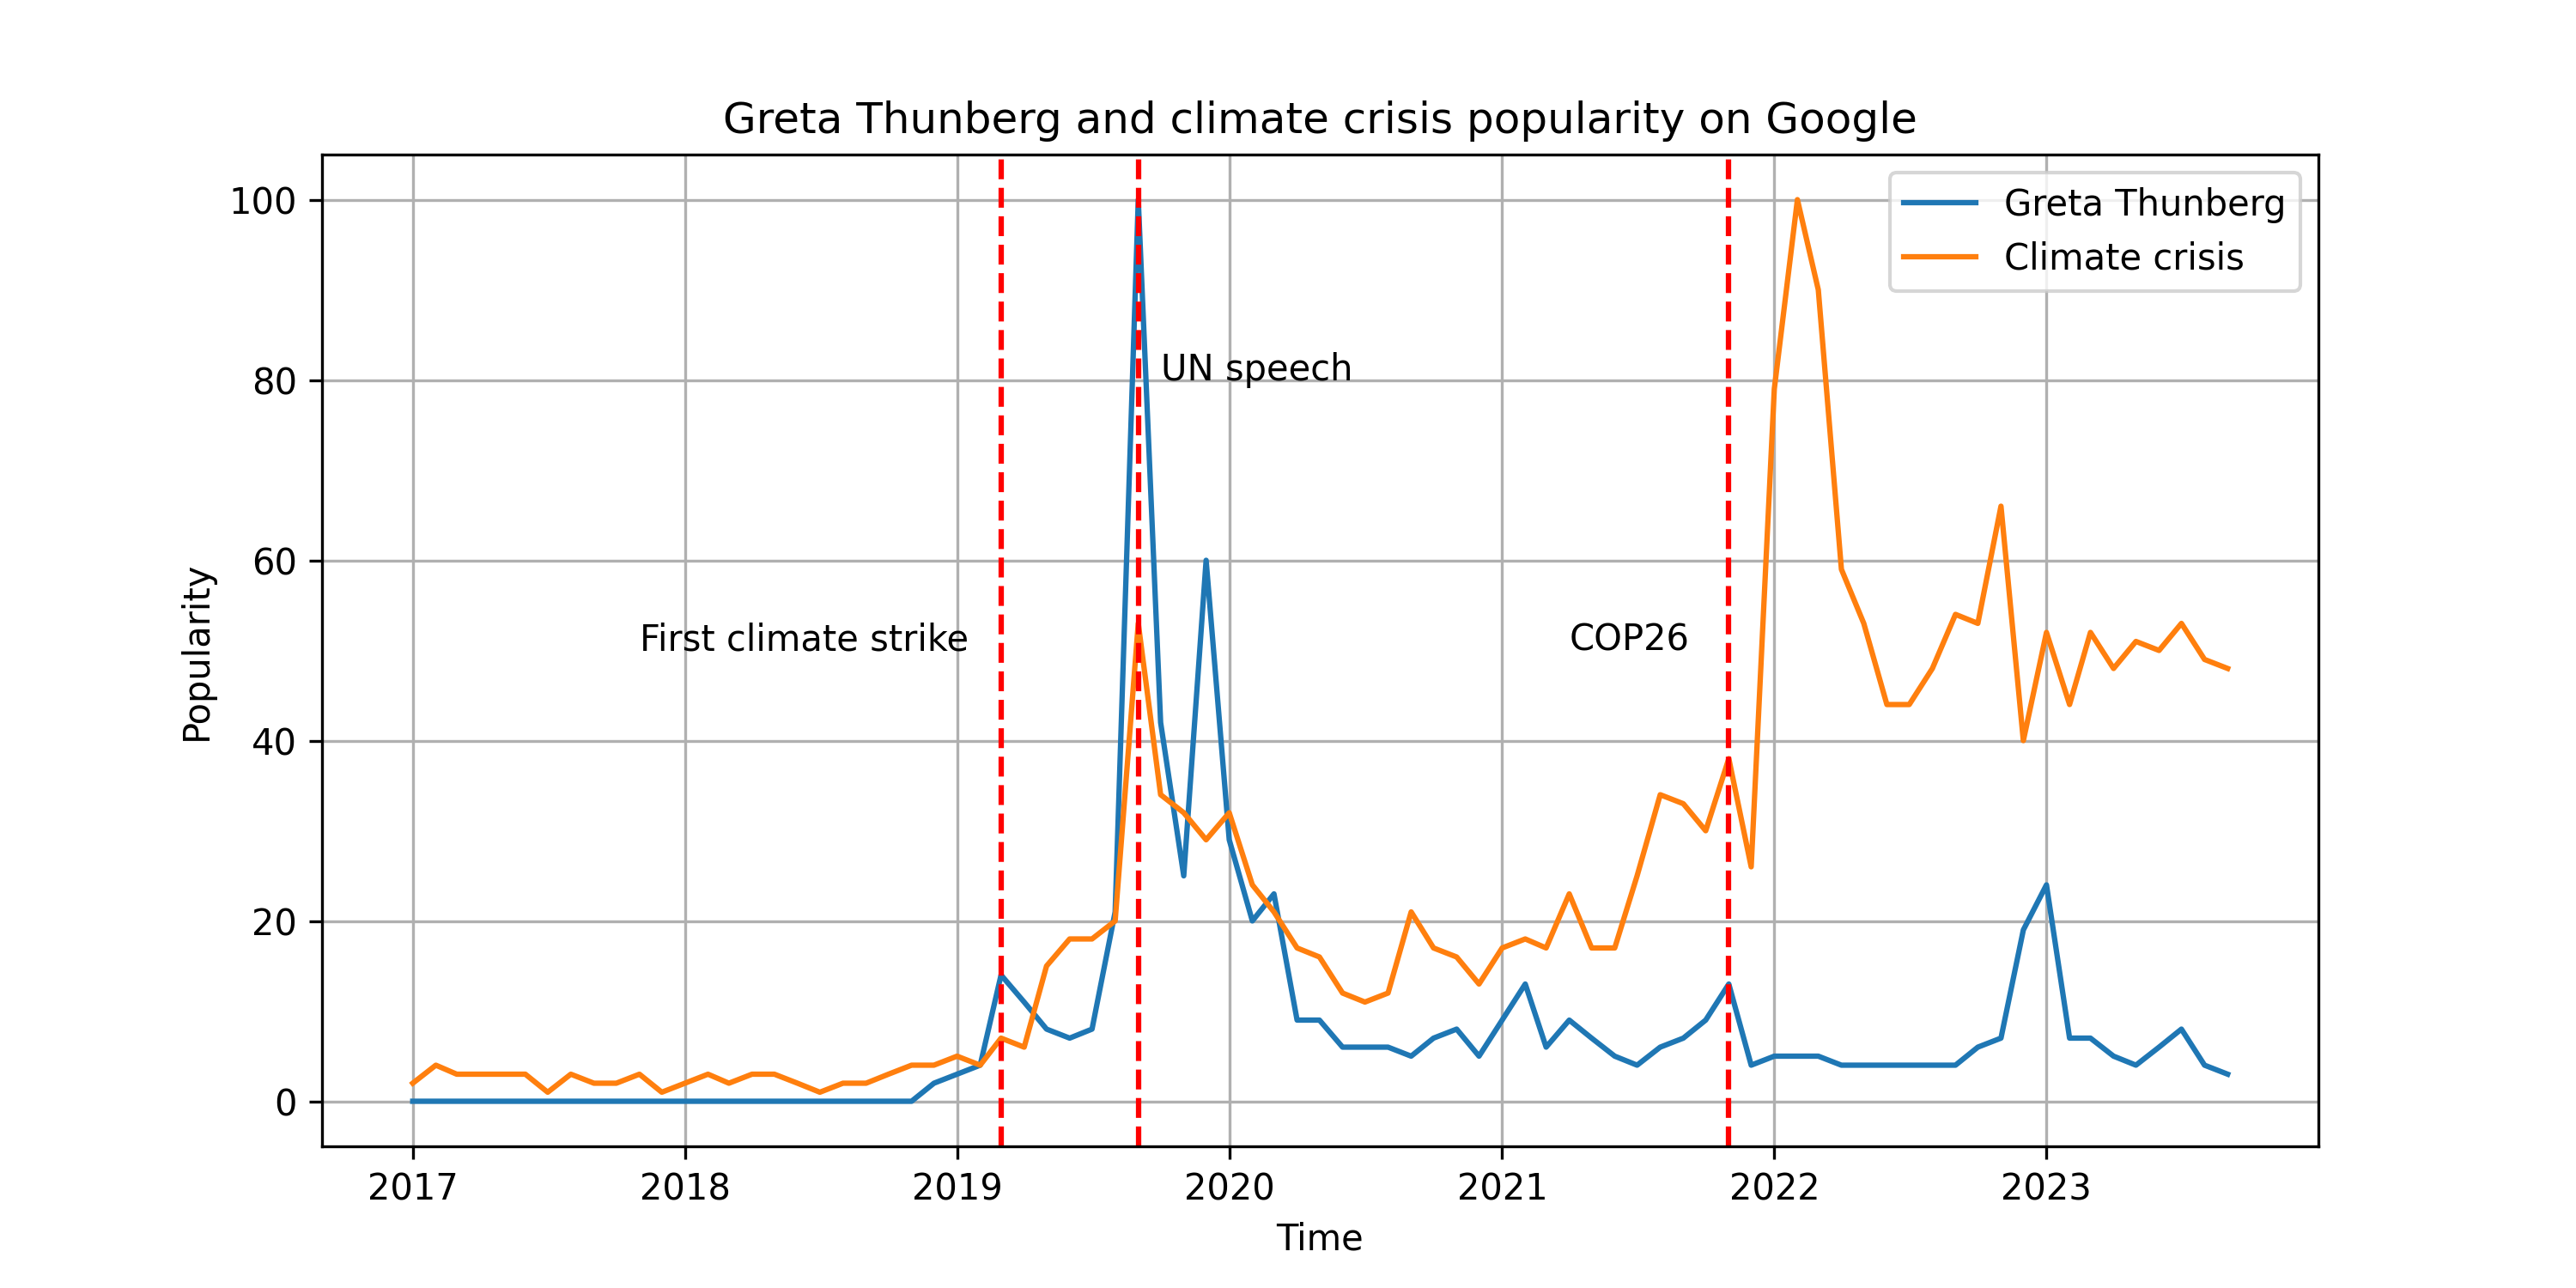
\includegraphics[width=0.85\linewidth]{Chapter1/figures/greta_climate_crisis.png}
    \caption{Interest on google over the time of Greta Thunberg and climat crisis}
    \label{fig:google_greta}
\end{figure}
In particular twitter is a place where political debate take place, and political events like 
Conference of Parties (COP) are the perfect joint between these two worlds because are the conferences where the highest political figures of many countries meet and talk about the climate emergencies. 



\paragraph{Conference of Parties}
Conferences of Parties are yearly conferences organized by United Nations where the topic of discussion is climate change, the first has been held in 1995 in Berlin, the most relevant are:
\begin{itemize}
    \item \textbf{COP3}: Kyoto protocol (1997)
    \item \textbf{COP21}: Paris agreement (2015)
    \item \textbf{COP26}: Glasgow Climate Pact (2021)
\end{itemize}

\\

For the first one unfortunatly we do not have twitter data but for the latter two we have, and our focus will be on that two .

In particular we will study the well known phenomenon among social scientist of polarization i.e. the tendency to choose one side of the political spectrum and stick with all their believes without trying to go outside their echo chamber.\\




This work lays its foundations on the research of Falkenberg et al \cite{falkenberg_growing_2022} where they discovered that the cop26 was way more polarized then cop21. Using a similar approach we will explore the ideological polarization topic by topic. 


\section{Research Questions}
Thanks to the structure we gave to our research we can now answer a new set of questions, related to the intratopic polarization, the first and most straightforward is RQ1 that has the goal to inspect the topics that are driving the polarization of the entire COP26. Consequently RQ2 wants to identify if these topics have always been so polarized or not.

Then we will move to some questions related to the users, in particular RQ3 want to see if the polarized users are polarized in the same way over the different topics or if there are topics in which they are in the opposite side of the spectrum. RQ4 instead investigate whether the users that talks about many different topics are more polarized than the user that are present in only one.

The last question instead (RQ5) looks into the possible cause of the growing polarization in the recent years, to see if the strikes that caused problems to the population created a negative feeling toward che cause. ( i don't know if include this because it's broad and i already have enought question)

\begin{enumerate}
    \item  Which are the most polarizing topics discussed on twitter during cop 26?
    \item how did topics evolved between cop21 and cop26?
    \item Is the single user polarization different across different topics? ( quelli a destra stanno  a destra in tutti i topic?)
    \item Are the users present in more topics polarized in different ways that the ‘experts’ that are present only in one or few topics?
    \item impact of Greta thunberg and climate strikes on polarization
\end{enumerate}






%********************************** %First Section  **************************************

\nomenclature[z-DEM]{DEM}{Discrete Element Method}
